\begin{tikzpicture}

\node[color=red] (1) at (1.5,3) {$X'$};
\node[color=blue] (2) at (1.5,2) {$X''$};
\node[color=black!60!green] (3) at (1.5,1) {$X'''$};

\coordinate (FirstCenter) at (7.4,3);
\coordinate (SecCenter) at (6.5,2);
\coordinate (ThirdCenter) at (7,1);

\draw [decorate,decoration={brace,amplitude=10pt}]
(1.2,0.9) -- (1.2,3.1) node [black,midway,xshift=-0.8cm] {$\mathbb{P}(X)$};

\draw[->,shorten >=0.3cm, color=red,thick,out=0,in=160] (1) to node [pos=0.2,fill=white] {$R(c, X')$} (FirstCenter) ;
\draw[->,shorten >=0.3cm, color=blue,thick,out=0,in=160] (2) to node [pos=0.2,fill=white] {$R(c, X'')$} (SecCenter) ;
\draw[->, shorten >=0.3cm, color=black!60!green,thick,out=0,in=160] (3) to node [pos=0.2,fill=white] {$R(c, X''')$} (ThirdCenter) ;

\draw[draw=none] (0,-2) -- (0,6) -- (10, 6) -- (10,-2);

\only<1>{%
\filldraw[color=red, fill opacity=0.2] (FirstCenter) circle (2.6);
\filldraw[color=blue, fill opacity=0.2] (SecCenter) circle (2.3cm);
\filldraw[color=black!60!green, fill opacity=0.2] (ThirdCenter) circle (2.7cm); }

\only<2>{%
\filldraw[color=red, fill opacity=0.2] (FirstCenter) circle (1.9cm);
\filldraw[color=blue, fill opacity=0.2] (SecCenter) circle (2cm);
\filldraw[color=black!60!green, fill opacity=0.2] (ThirdCenter) circle (2.2cm); }

\only<3>{%
\filldraw[color=red, fill opacity=0.2] (FirstCenter) circle (1.5cm);
\filldraw[color=blue, fill opacity=0.2] (SecCenter) circle (1.2cm);
\filldraw[color=black!60!green, fill opacity=0.2] (ThirdCenter) circle (1.4cm); }

\only<4>{%
\filldraw[color=red, fill opacity=0.2] (FirstCenter) circle (0.7cm);
\filldraw[color=blue, fill opacity=0.2] (SecCenter) circle (0.5cm);
\filldraw[color=black!60!green, fill opacity=0.2] (ThirdCenter) circle (0.6cm); }

\only<5>{%
\filldraw[color=red, fill opacity=0.2] (FirstCenter) circle (0.2cm);
\filldraw[color=blue, fill opacity=0.2] (SecCenter) circle (0.3cm);
\filldraw[color=black!60!green, fill opacity=0.2] (ThirdCenter) circle (0.25cm); }

\only<1-6>{%
\filldraw[color=red] (FirstCenter) circle (0.1cm);
\filldraw[color=blue] (SecCenter) circle (0.1cm);
\filldraw[color=black!60!green] (ThirdCenter) circle (0.1cm); }

\node[align=center] at (1,4.5) {Data \\ Inputs};
\node[align=center] at (4,4.5) {Solving \\ (Approximating)};
\node[align=center] at (8,4.5) {Optimal Solutions \\ (Approx. Sets)};
\only<2->{%
\node[align=center] at (7,-1) {Increasing $\beta$ (decreasing $\gamma$) \\
Extracts more information from input.};}
\end{tikzpicture}